% Winners
%	Best Gradients
%	Best non-Gradients
% Losers
%	Why it didn't work
\noindent\textbf{General Trends}\newline

	We expected each participant to rank their own layout as superior to the others.
	Each wake model accounts for different fluids phenomena, and what one wake model considers an optimal layout, another may not.
	An example of this would be if one participant used Larsen's Dynamic Meandering Wake (DMW)\cite{Larsen2007}, depicted in \cref{fig:dmw}.
	A turbine placed downstream, slightly offset to miss the wake oscilations accounted for in DMW would, under another wake model not accounting for this ``meander'' (such the Jensen's model\cite{Jensen1983}), feel the full brunt of the wake, and deliver a sub-optimal AEP.

	\begin{figure}[H]
		\centering
			\begin{subfigure}{.5\textwidth}
			  \centering
			  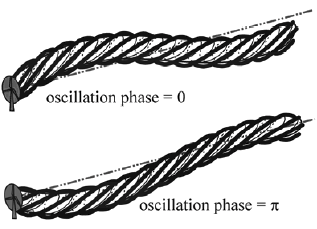
\includegraphics[width=.7\linewidth]{./figures/MeanderingWakeSpace(Larsen2007).png}
			  \caption{DMW depicted 3-dimensionally}
			  \label{fig:LarsenDMW3d}
			\end{subfigure}%
			\begin{subfigure}{.5\textwidth}
			  \centering
			  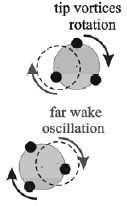
\includegraphics[width=.3\linewidth]{./figures/MeanderingWakeTrefftz(Larsen2007).png}
			  \caption{DMW in the Trefftz plane}
			  \label{fig:LarsenDMWTrefftz}
			\end{subfigure}
			\caption{Sketch of Larsen's Dynamic Meandering Wake (DMW) behind a wind turbine \cite{Larsen2007}.}
			\label{fig:dmw}
			\vspace{-10pt}
	\end{figure}

	Unexpectedly, only \textit{par4} and \textit{par5} found their own layouts to be superior to the other participants.
	Furthermore, all other participants also found \textit{par4} and \textit{par5}'s layouts superior to their own, though to varying degrees.
	3 particiants (including self-reporting) found \textit{par4} to have the highest AEP producing layout.
	The other two participants found \textit{par5} to have the highest AEP producing layout.
	% Visual representations

\subsubsection{Analysis of Best Results}

	Within expectations, \textit{par4} and \textit{par5} ranked their own layouts superior to all other participant results.
	Two correlations are important to note regarding \textit{par4} and \textit{par5}.
	Firstly, both used variations of the same wake model.
	From CAse Study 1, \textit{par5} used the simplified Gaussian wake model previously described\cite{Bastankhah2016,Thomas2018}.
	Though \textit{par4} also used the Gaussian wake model \cite{Bastankhah2016}, \textit{par4} combined it with the wake model created by Niayifar and Porté-Agel \cite{Niayifar2016}, supplemented by the WEC method described earlier.
	Furthermore \textit{par4} also accounted for partial wake, shear, ambient turbulence intensity, and local turbulence intensity.
	None of these factors were accounted for by \textit{par5}.
	The second factor to note is that despite using very similar wake models, \textit{par4} and \textit{par5} used different gradient-based optimization algorithms that nonetheless reached very similar conclusions.

	As can be seen in the visual depictions included later in \cref{app:cs2-layouts}, \textit{par4} and \textit{par5} found nearly identical optimal turbine placements.
	Though pictorally appearing identical, the actual coordinates do indeed differ, enough so to result in different AEP calculations shown in the tables above.

	Without LES data, the conclusions able to be drawn from the cross-comparison analysis are limited.
	That both \textit{par4} and \textit{par5} were found by the other participant wake models to have superior placement could be a result of either a more efficient optimization method, or a better coupling between optimization method and wake model.
	That these minima existed within the other wake models (resulting in a higher computed AEP by those models) yet were nevertheless undiscovered in their optimizations, is inconclusive in telling us which it is.

	Both \textit{par4} and \textit{par5} used similar wake models, but very different optimization methods.
	Coding in MATLAB, \textit{par5} did 1000 random starts, and used MATLAB's built in FMINCON() (which uses a finite difference method to find gradients) to optimize for a minimum.
	Using a combination of Python, FORTRAN, and Bash, \textit{par4} ran 1 ordered with 199 random starts for 200 optimizations altogether.
	SNOPT's SQP algorithm was \textit{par4}'s implemented optimizer.

	Of note, from trends seen above in Case Study 1, \textit{par5}'s optimization methods demostrate superior performance for small design variable sizes, but comparitively degrades as the windfarm size increases.
	The superior performance of this wake model and optimization method combination for this small farm may not be reproducable for farms of even larger sizes than those tested.

\subsubsection{Analysis of Worst Results}

	Again, conlusions able to be drawn from the cross-comparison analysis are limited due to the lack of LES data.
	Suprisingly, however, \textit{par2}'s results were found by every other participant to be inferior, even by \textit{par2}.
	As noted earlier, this could be a result of either poor wake model pairing with optimization method, or simply an optimization method shortcoming.
	Using data from Case Study 1, \textit{par2}'s optimization method shows inferior results for small sample sizes, but increases in comparative performance as wind farm size and number of design variables increase.
	That data leads us to believe the inferior performance here is a product of the wind farm size, and not a poor pairing of wake model with optimization method.
	However, both the LES analysis and attempts at farms of larger sizes would need to be analyzed to find a definitive conclusion. 

	Discounting the two universal top performers (\textit{par4} and \textit{par5}), \textit{par1}'s results were more in line with what we expected from the cross-comparison.
	Namely, that \textit{par1} found its layout superior to the others, but that the others did not find it so.
	%The LES will need to be run to determine how \textit{par1}'s wake model compares to the others.

\subsubsection{Discussion}

	A weakness voiced by participants of earlier case studies are scenarios where non-novel, and simplistic layouts (such as all turbines on the boundary border) are optimal.
	The small farm radius with few turbines given for this case study seems to have unknowingly fallen into this category.
	What is interesting, however, is that three of the five participants were trapped in local optima, and proved blind to optima others found, using different physics approximations and optimization methods.
	This could be a result of inferior optimization methods, lack of sufficient iterations, lack of sufficient wall time, or a combination of factors.

	%Border placement of turbines in concentric rings was supplied for the three wind farm sizes in case study 1, created from intuition.
	%As an unintended validation, all participants of case study 2 reported layouts following this same pattern applied to this smaller farm size, despite being results of random starting locations.
	%This confirms the hypothesis that, for small farm sizes, border placement and concentric rings will tend to deliver optimal farm AEP.